%% WP: Deeply Embedded / Smart Pointer / Reference Counting
\documentclass{beamer}
\usepackage[utf8]{inputenc}
\usepackage{listings}
\usepackage{graphicx}
\usepackage{lmodern}
\usepackage{default}

\usetheme{AnnArbor}
\usecolortheme{crane}

\title{Smart Pointer \& Reference Counting}

\author{
  Marian Triebe\\
  \tiny \texttt{marian.triebe@haw-hamburg.de}
}
\date{} % Kein Datum
\subtitle{WP Deeply Embedded Sommer Semester 2015}

\definecolor{eclipse-violet}{rgb}{0.50, 0.0, 0.46}
\definecolor{eclipse-green}{rgb}{0.25, 0.50, 0.37}
\definecolor{eclipse-blue}{rgb}{0.17, 0.0, 1.00}
\lstset{
  language=C++,
  showstringspaces=false,
  basicstyle=\ttfamily\small\scriptsize,
  keywordstyle=\bfseries\color{eclipse-violet},
  commentstyle=\color{eclipse-green},
  stringstyle=\color{eclipse-blue},
  breaklines=true
}

\begin{document}

% Titel
\begin{frame}
 \titlepage
\end{frame}
 
% Themenübersicht
\begin{frame}
 \frametitle{Themen}
 \begin{itemize}
  \item Motivation
  \item Shared Pointer (Smart Pointer)
  \item Shared Pointer und Arrays
  \item Intrusive Pointer (Reference Counting)
  \item Implementierung von Shared Pointern
 \end{itemize}
\end{frame}

% Motivation
\begin{frame}
 \frametitle{Motivation}
 \begin{itemize}
 	\item Keine Garbage Collection (GC) in C++
 	\item Häufige Fehler: Memory Leaks, Use-after-free
 	\item Motivation: Prüfen ob Objekte noch benötigt werden ohne
 	Performance-Verlust
 \end{itemize}
\end{frame}


% Boost vs STL Pointer
\begin{frame}
 \frametitle{Shared Pointer}
 \begin{itemize}
  \item Boost Pointer
  \item STL Pointer
  \item Sind größtenteils per Textersetzung austauschbar
  \item Kamen zuerst nach boost, später in STL
 \end{itemize}
\end{frame}

% Basics
\begin{frame}
  \frametitle{Die Basics}
  \begin{itemize}
    \item RAW Pointer \textit{int* p = new int(2);}
    \item Smart Pointer als Wrapper um RAW Pointer
    %\item Für Arrays die passende \textit{\_array} Klasse verwenden
    \item Dynamisch allokierter Speicher liegt auf dem Heap
    \item Frage: Ist der Unterschied zwischen Heap und Stack bewusst?
  \end{itemize}	
\end{frame}

% Scoped/Unique Pointer
\begin{frame}[fragile]
 \frametitle{Scoped / Unique Pointer}
 \begin{itemize}
  %\item Umsetzung von RAII für dynamisch allokierten Speicher
  %\item Als Wrapper um RAW-Pointer
  \item Speicherfreigabe sobald Scope des "Owners" verlassen wird
  \item Nicht kopierbar
  \item Transfer of ownership \tiny (nur \textit{unique\_ptr} mit \textit{std::move})
  \item \normalsize Deleter Funktion nur bei \textit{unique\_ptr}
 \end{itemize}
 Implementierungen:
 \begin{itemize}
 	\item \textit{std::unique\_ptr} in STL
 	\item \textit{boost::scoped\_ptr} in boost
 \end{itemize}
 Jedoch unterscheiden sich beide voneinander
\end{frame}

% Scoped/Unique Pointer
\begin{frame}
 \frametitle{Scoped / Unique Pointer}
 \begin{itemize}
  \item Wann sollte \textit{boost::scoped\_ptr} verwendet werden?
   \begin{itemize}
 	\item Bei komplexerem Programflow mit mehreren Return Punkten
   \end{itemize}
  \item Wann sollte \textit{std::unique\_ptr} verwendet werden?
  \begin{itemize}
   \item Wenn bspw. mit einer Bibliothek gearbeitet wird, die bei Aufruf Speicher allokiert
   \item Kann auch wie \textit{boost::scoped\_ptr} genutzt werden
   \item Zusätzliche Möglichkeit des Transfer of Ownership
  \end{itemize}
 \end{itemize}
\end{frame}

% Beispiel scoped_ptr (boost)
\begin{frame}[fragile]
 \frametitle{boost::scoped\_ptr Beispiel}
 \begin{lstlisting}
#include <iostream>
#include "boost/scoped_ptr.hpp"
using namespace std;

struct mystruct {
  mystruct() { cout << __PRETTY_FUNCTION__ << endl; }
  ~mystruct() { cout << __PRETTY_FUNCTION__ << endl; }
};

int main() {
  {
    boost::scoped_ptr<mystruct> ptr(new mystruct);
    // hier kann ptr benutzt werden
    // ...
  }
  return 0;
}
 \end{lstlisting}
\end{frame}

% Beispiel unique_ptr (STL) Ownership move
\begin{frame}[fragile]
 \frametitle{unique\_ptr Beispiel (Transfer of Ownership)}
 \begin{lstlisting}
#include <iostream>
#include <memory>
struct Foo {
    Foo() { std::cout << "Foo::Foo\n"; }
    ~Foo() { std::cout << "Foo::~Foo\n"; }
    void bar() { std::cout << "Foo::bar\n"; }
};
void f(const Foo &foo) { std::cout << "f(const Foo&)\n"; }
int main()
{
    std::unique_ptr<Foo> p1(new Foo);  // p1 owns Foo
    if (p1) { p1->bar(); }
    {
        std::unique_ptr<Foo> p2(std::move(p1));  // now p2 owns Foo
        f(*p2);
        p1 = std::move(p2);  // ownership returns to p1
        std::cout << "destroying p2...\n";
    }
    if (p1) { p1->bar(); }
    // Foo instance is destroyed when p1 goes out of scope
}
 \end{lstlisting}
 \tiny Geklaut von http://en.cppreference.com/w/cpp/memory/unique\_ptr
 \normalsize
\end{frame}

% Beispiel unique_ptr (STL)
\begin{frame}[fragile]
 \frametitle{std::unique\_ptr Beispiel}
 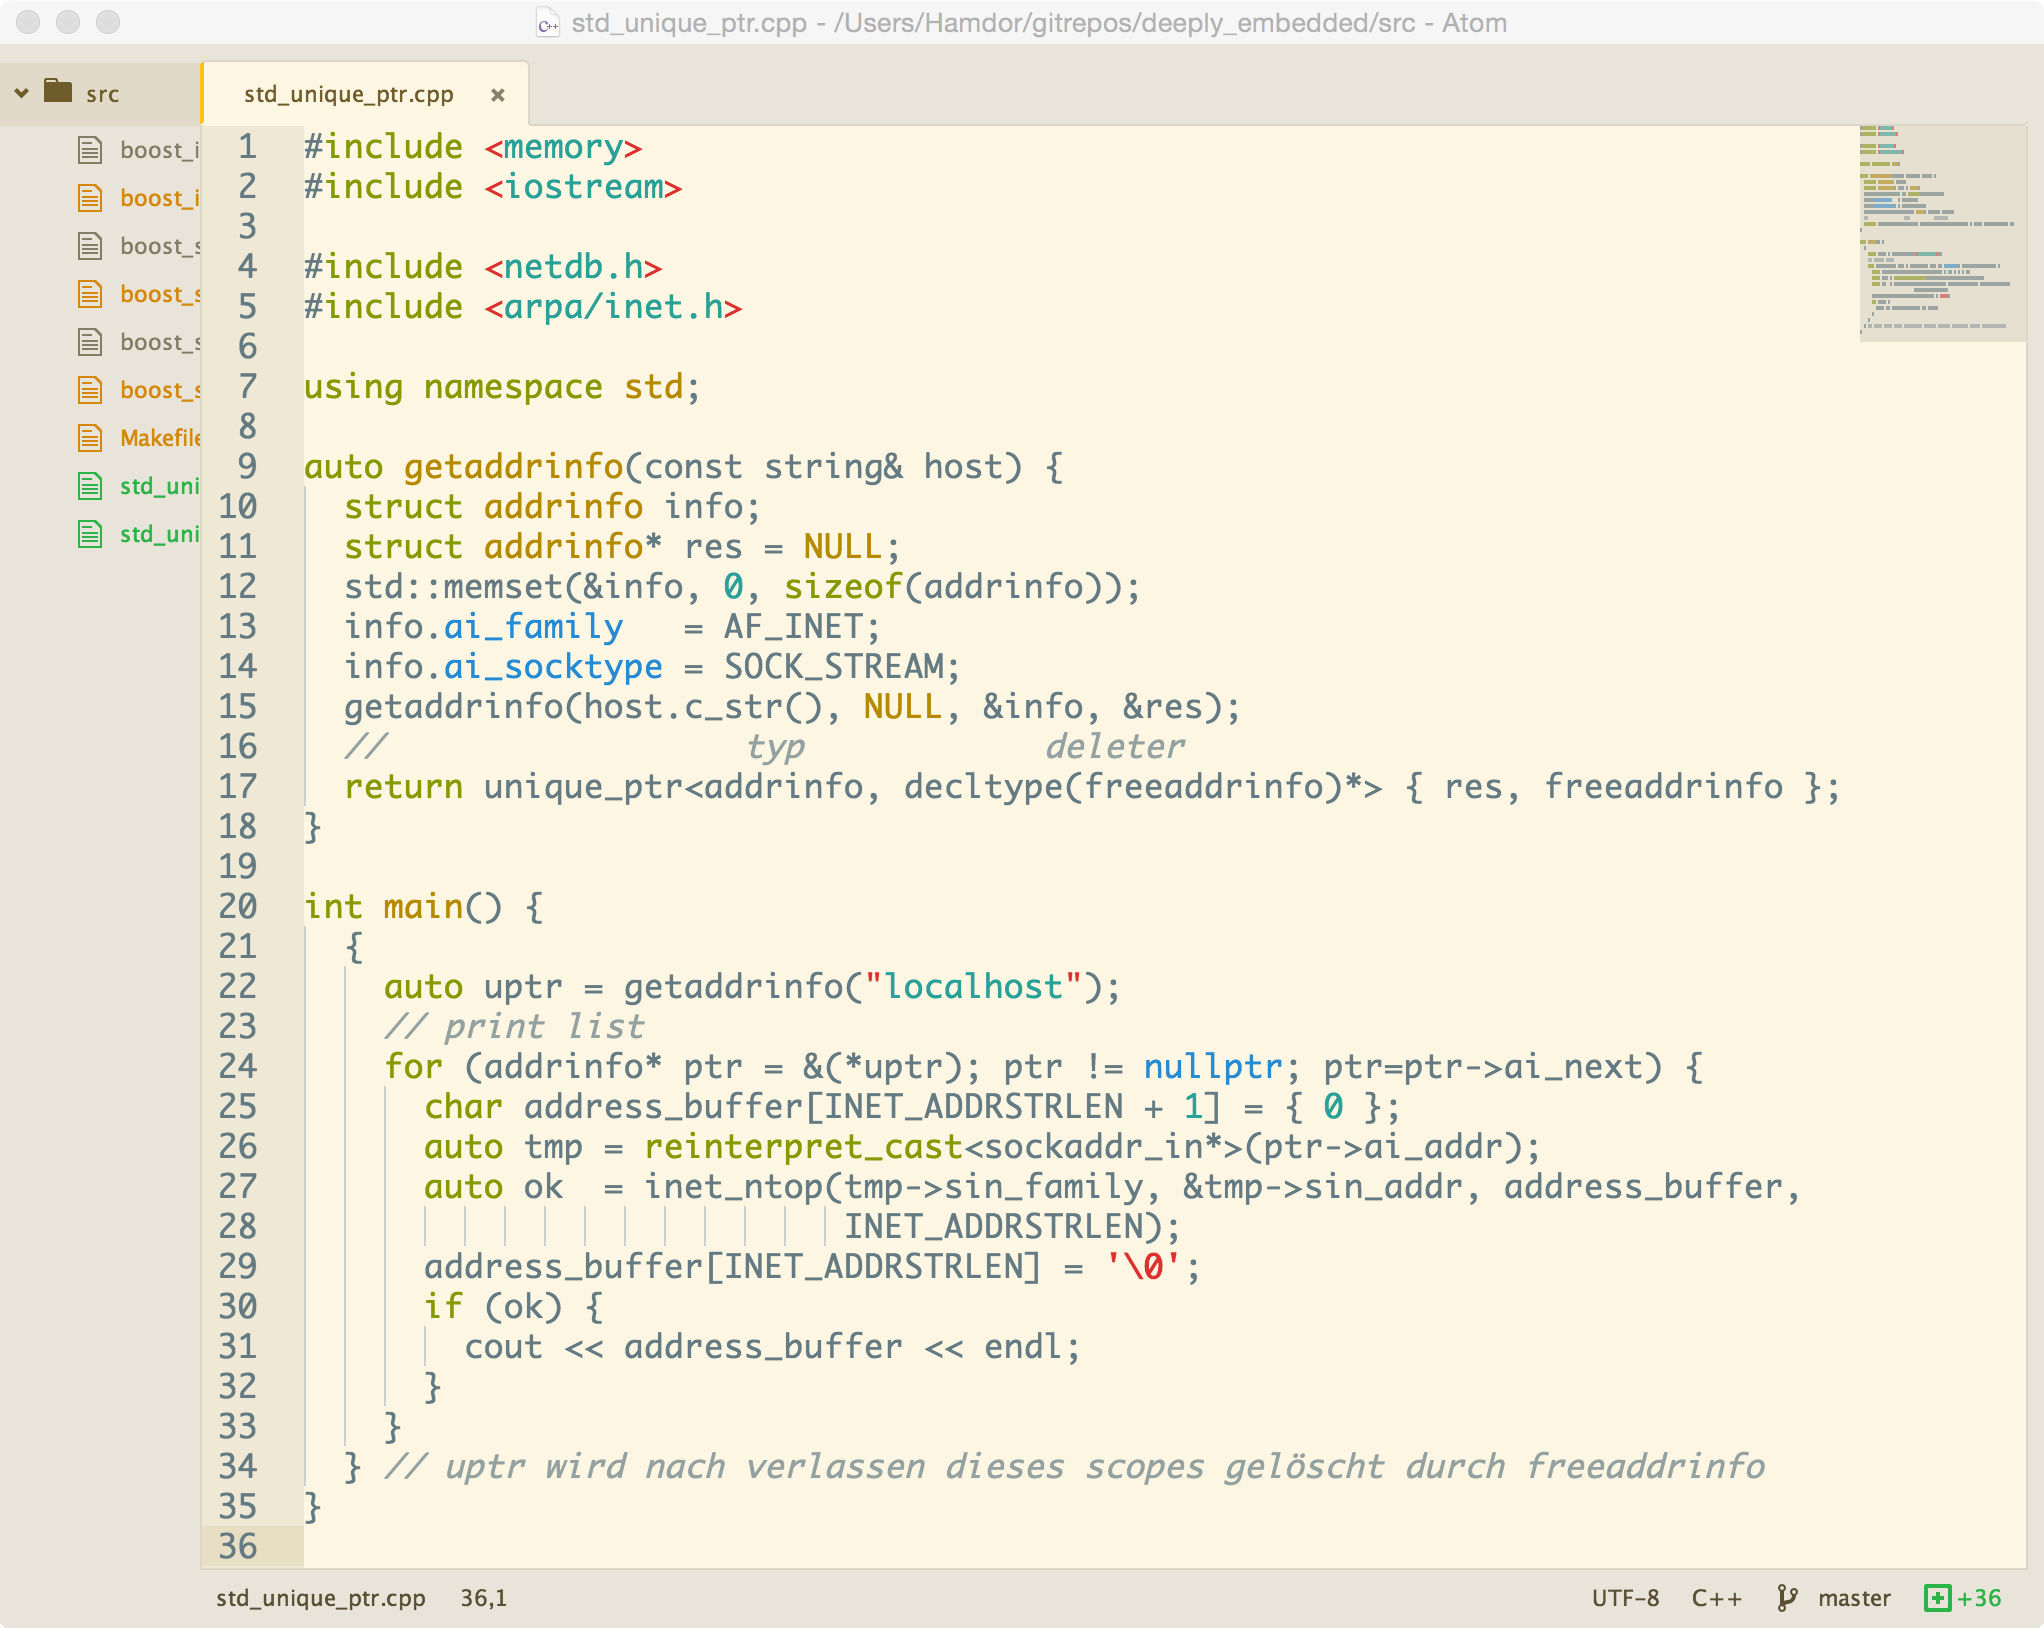
\includegraphics[scale=.265]{unique_ptr_usage}
\end{frame}

% Shared Pointer
\begin{frame}
 \frametitle{Shared Pointer}
 \begin{itemize}
  \item Sobald keine Shared Pointer mehr auf Speicher verweisen, wird Objekt gelöscht
  \item Nicht kopierbar
  \item Kein transfer of ownership (per \textit{std::move})
  \item Per Funktionsaufruf von \textit{make\_shared} erstellbar
 \end{itemize}
 Implementierungen:
 \begin{itemize}
 	\item \textit{std::shared\_ptr}
 	\item \textit{boost::shared\_ptr}
 \end{itemize}
\end{frame}

% Shared Pointer Beispiel
\begin{frame}[fragile]
  \frametitle{Shared Pointer Beispiel}
  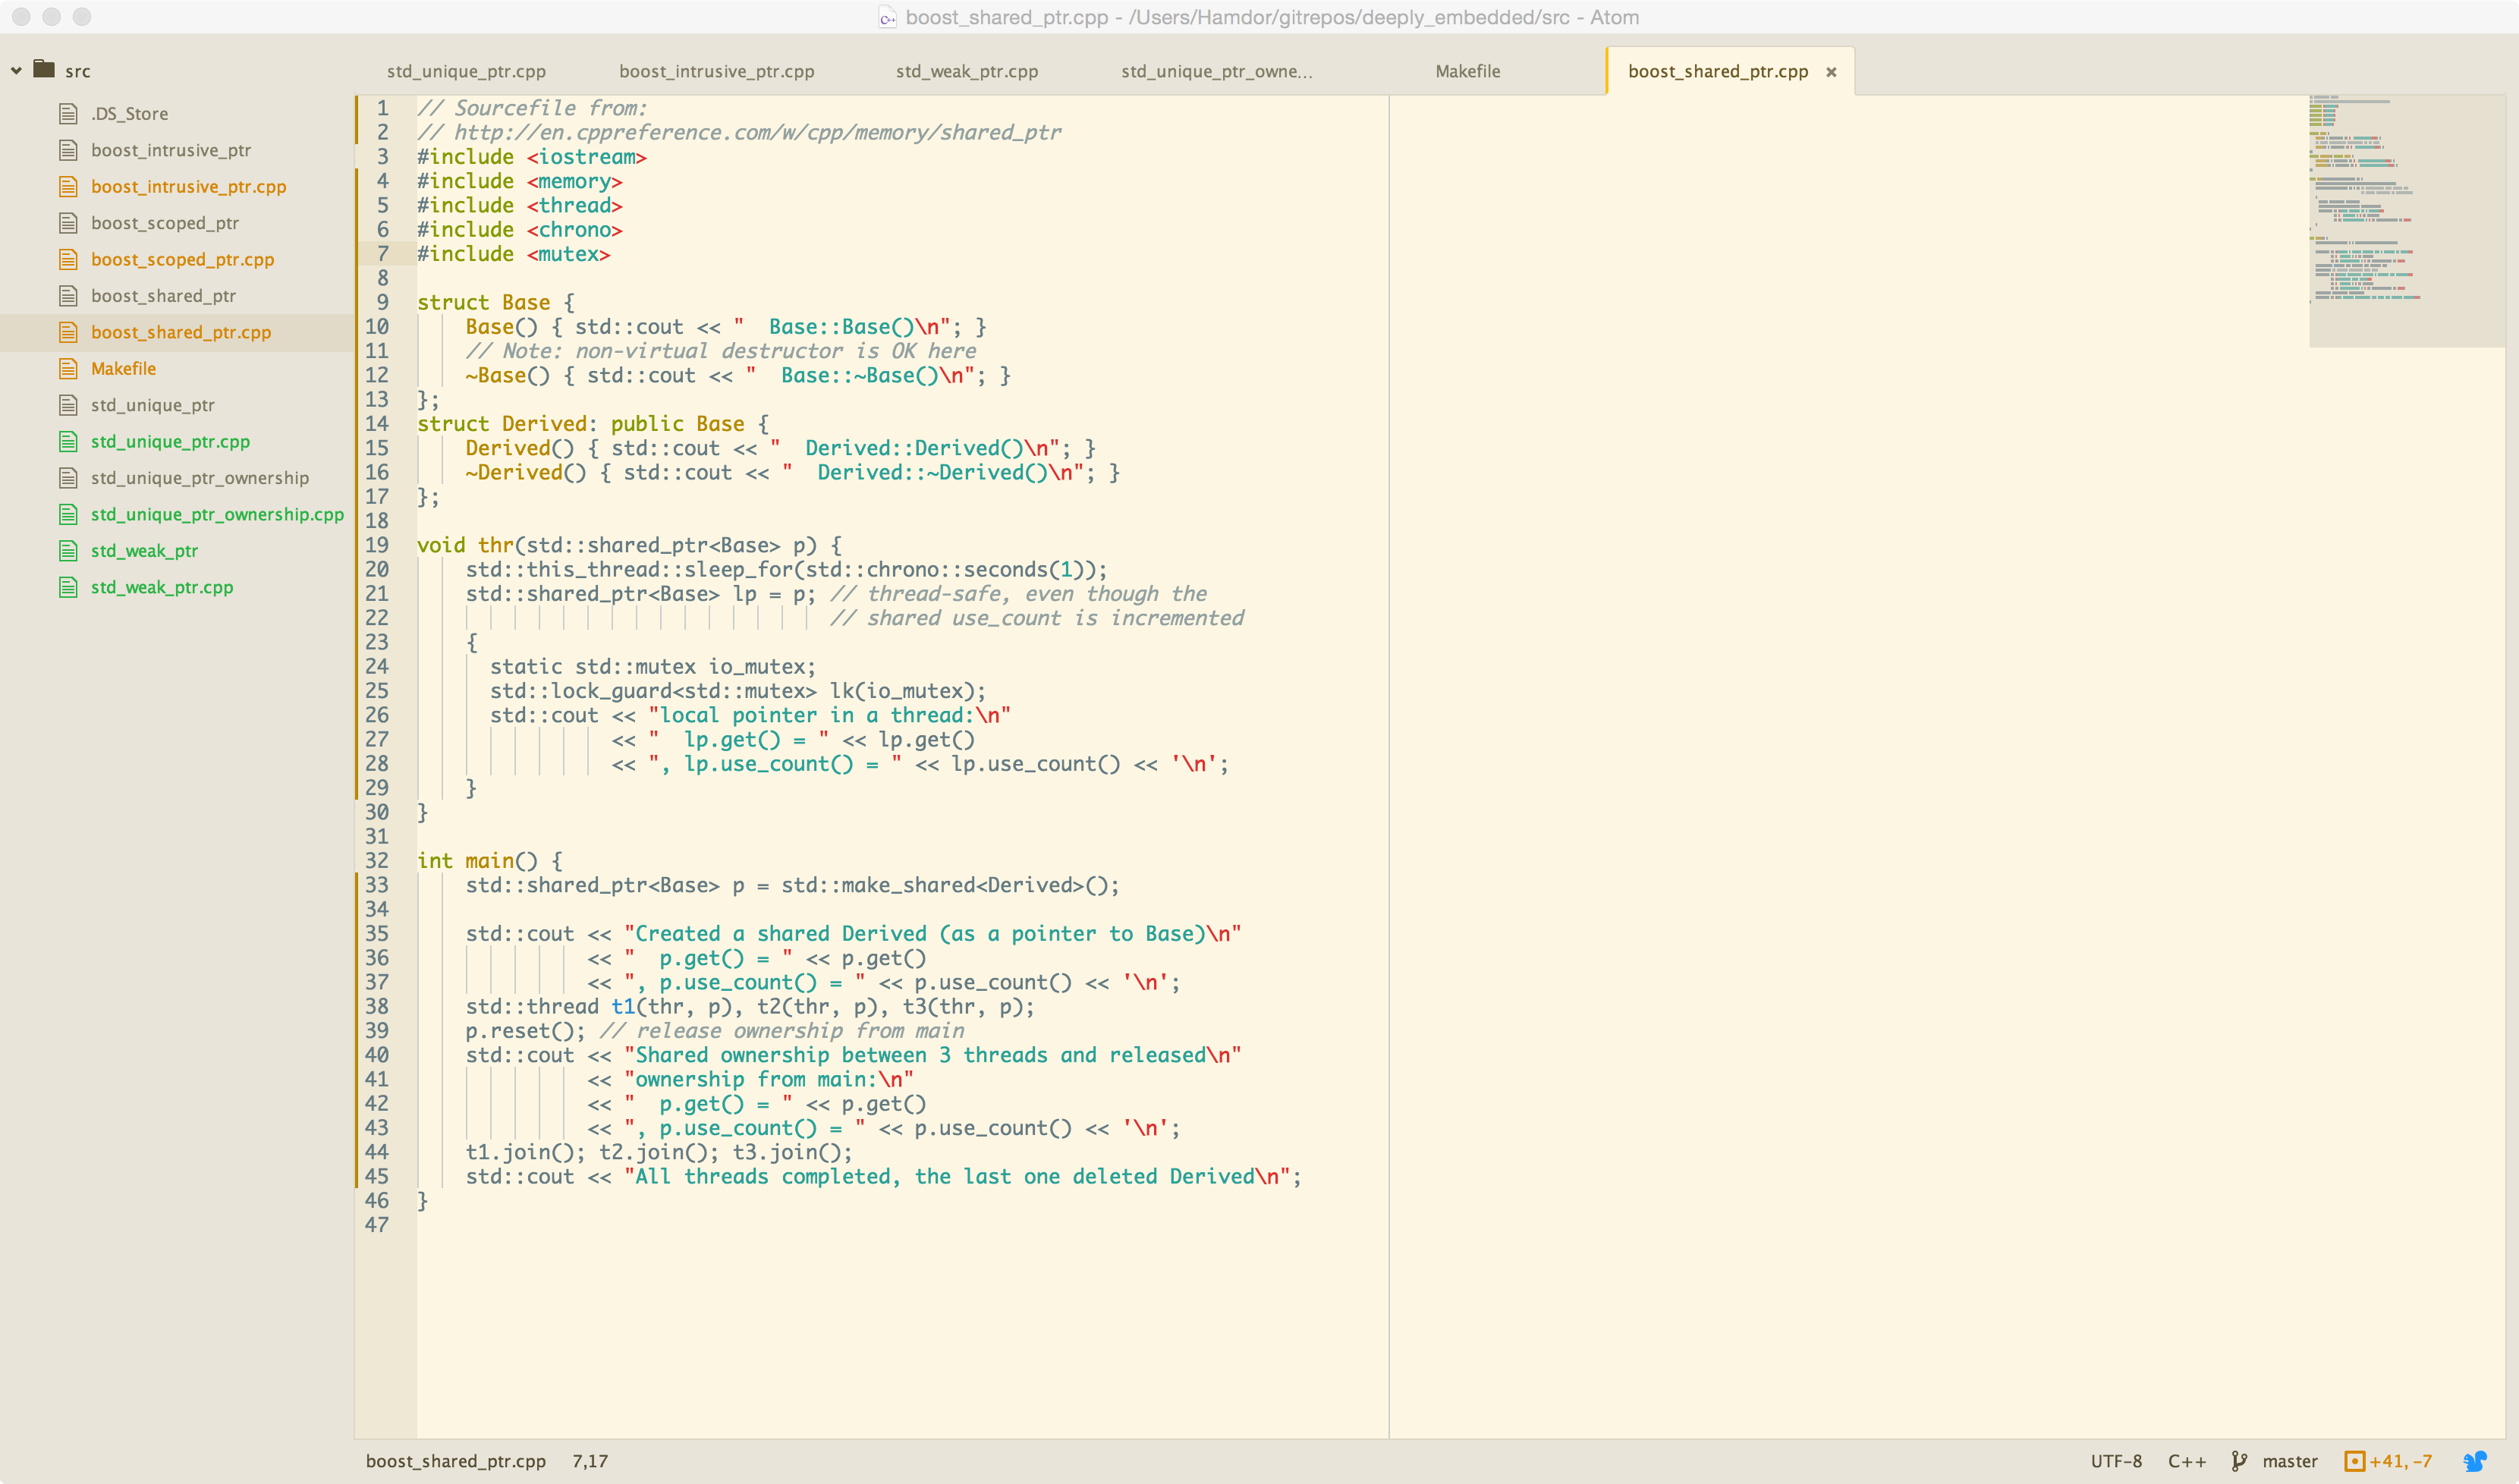
\includegraphics[scale=.2]{shared_ptr_usage}
\end{frame}

% Weak Pointer
\begin{frame}[fragile]
 \frametitle{Weak Pointer}
 \begin{itemize}
  \item Kann aus einem \textit{shared\_ptr} erstellt werden
  \item Erhöht nicht den Referenzzähler (also nicht wie \textit{shared\_ptr})
  \item Kann einen \textit{shared\_ptr} erstellen %\textit{(per `lock()` oder shared\_ptr Konstruktor)}
 \end{itemize}
 Implementierungen:
 \begin{itemize}
 	\item \textit{std::weak\_ptr}
 	\item \textit{boost::weak\_ptr}
 \end{itemize}
\end{frame}

% Wann sollte shared_ptr verwendet werden?
\begin{frame}
 \frametitle{Wann sollte shared\_ptr oder weak\_ptr verwendet werden?}
 \begin{itemize}
  \item shared\_ptr
  \begin{itemize}
   \item Ist verantwortlich für das löschen des Objektes
   \item Nicht definiertes Verhalten, wenn Objekt nicht existiert
   \item Es muss sichergestellt werden, dass das Objekt existiert
  \end{itemize}
  \item weak\_ptr
  \begin{itemize}
   \item Wenn nicht verantwortlich für löschen des Objektes
   \item Definiertes Verhalten, wenn Objekt nicht existiert
  \end{itemize}
 \end{itemize}
\end{frame}

% Shared Pointer und Arrays
\begin{frame}[fragile]
\frametitle{Shared Pointer und Arrays}
\begin{itemize}
	\item \textit{boost::shared\_ptr} kann erst ab Version 1.53 für Arrays verwendet werden
	\item \textit{std::shared\_ptr} kann immer für Arrays verwendet werden
	\item Jedoch muss ein \textit{custom deleter} verwendet werden
\end{itemize}
\begin{lstlisting}
// Array mit 20 Ints,    allokation         custom deleter
std::shared_ptr<int> sp(new int[20], std::default_delete<int[]>());

// Custom deleter kann auch per Lambda spezifiziert werden
std::shared_ptr<int> sp(new int[20], [](int* p) { delete[] p; } );

// Unique PTR ruft automatisch korrekten deleter auf
std::unique_ptr<int[]> uptr(new int[20]);
\end{lstlisting}
\end{frame}

\begin{frame}[fragile]
 \frametitle{weak\_ptr Beispiel}
 \begin{lstlisting}
#include <iostream>
#include <memory>

std::weak_ptr<int> gw;

void f() {
  if (auto spt = gw.lock()) {
	std::cout << *spt << "\n";
  } else {
    std::cout << "gw is expired\n";
  }
}

int main() {
  {
    auto sp = std::make_shared<int>(42);
  	gw = sp;
  	f();
  }
  f();
}
 \end{lstlisting}
 \tiny Geklaut von http://en.cppreference.com/w/cpp/memory/weak\_ptr
\end{frame}

% boost::intrusive_ptr
\begin{frame}[fragile]
 \frametitle{boost::intrusive\_ptr}
 \begin{itemize}
   \item Referenzzähler in Klasse eingebaut \tiny (oft durch Vererbung/Interface)\normalsize
   \item Referenzzähler ist normaler unsigned Integer
   \item Gleichviel Speicherverbrauch wie RAW-Pointer
   \item Kein Overhead (im Vergleich zum \textit{shared\_ptr})
   \item Wird auch oft ohne Boost implementiert, damit keine Boost-dependency
 \end{itemize}
\end{frame}

% boost::intrusive_ptr Beispiel
\begin{frame}
 \frametitle{boost::intrusive\_ptr Beispiel}
 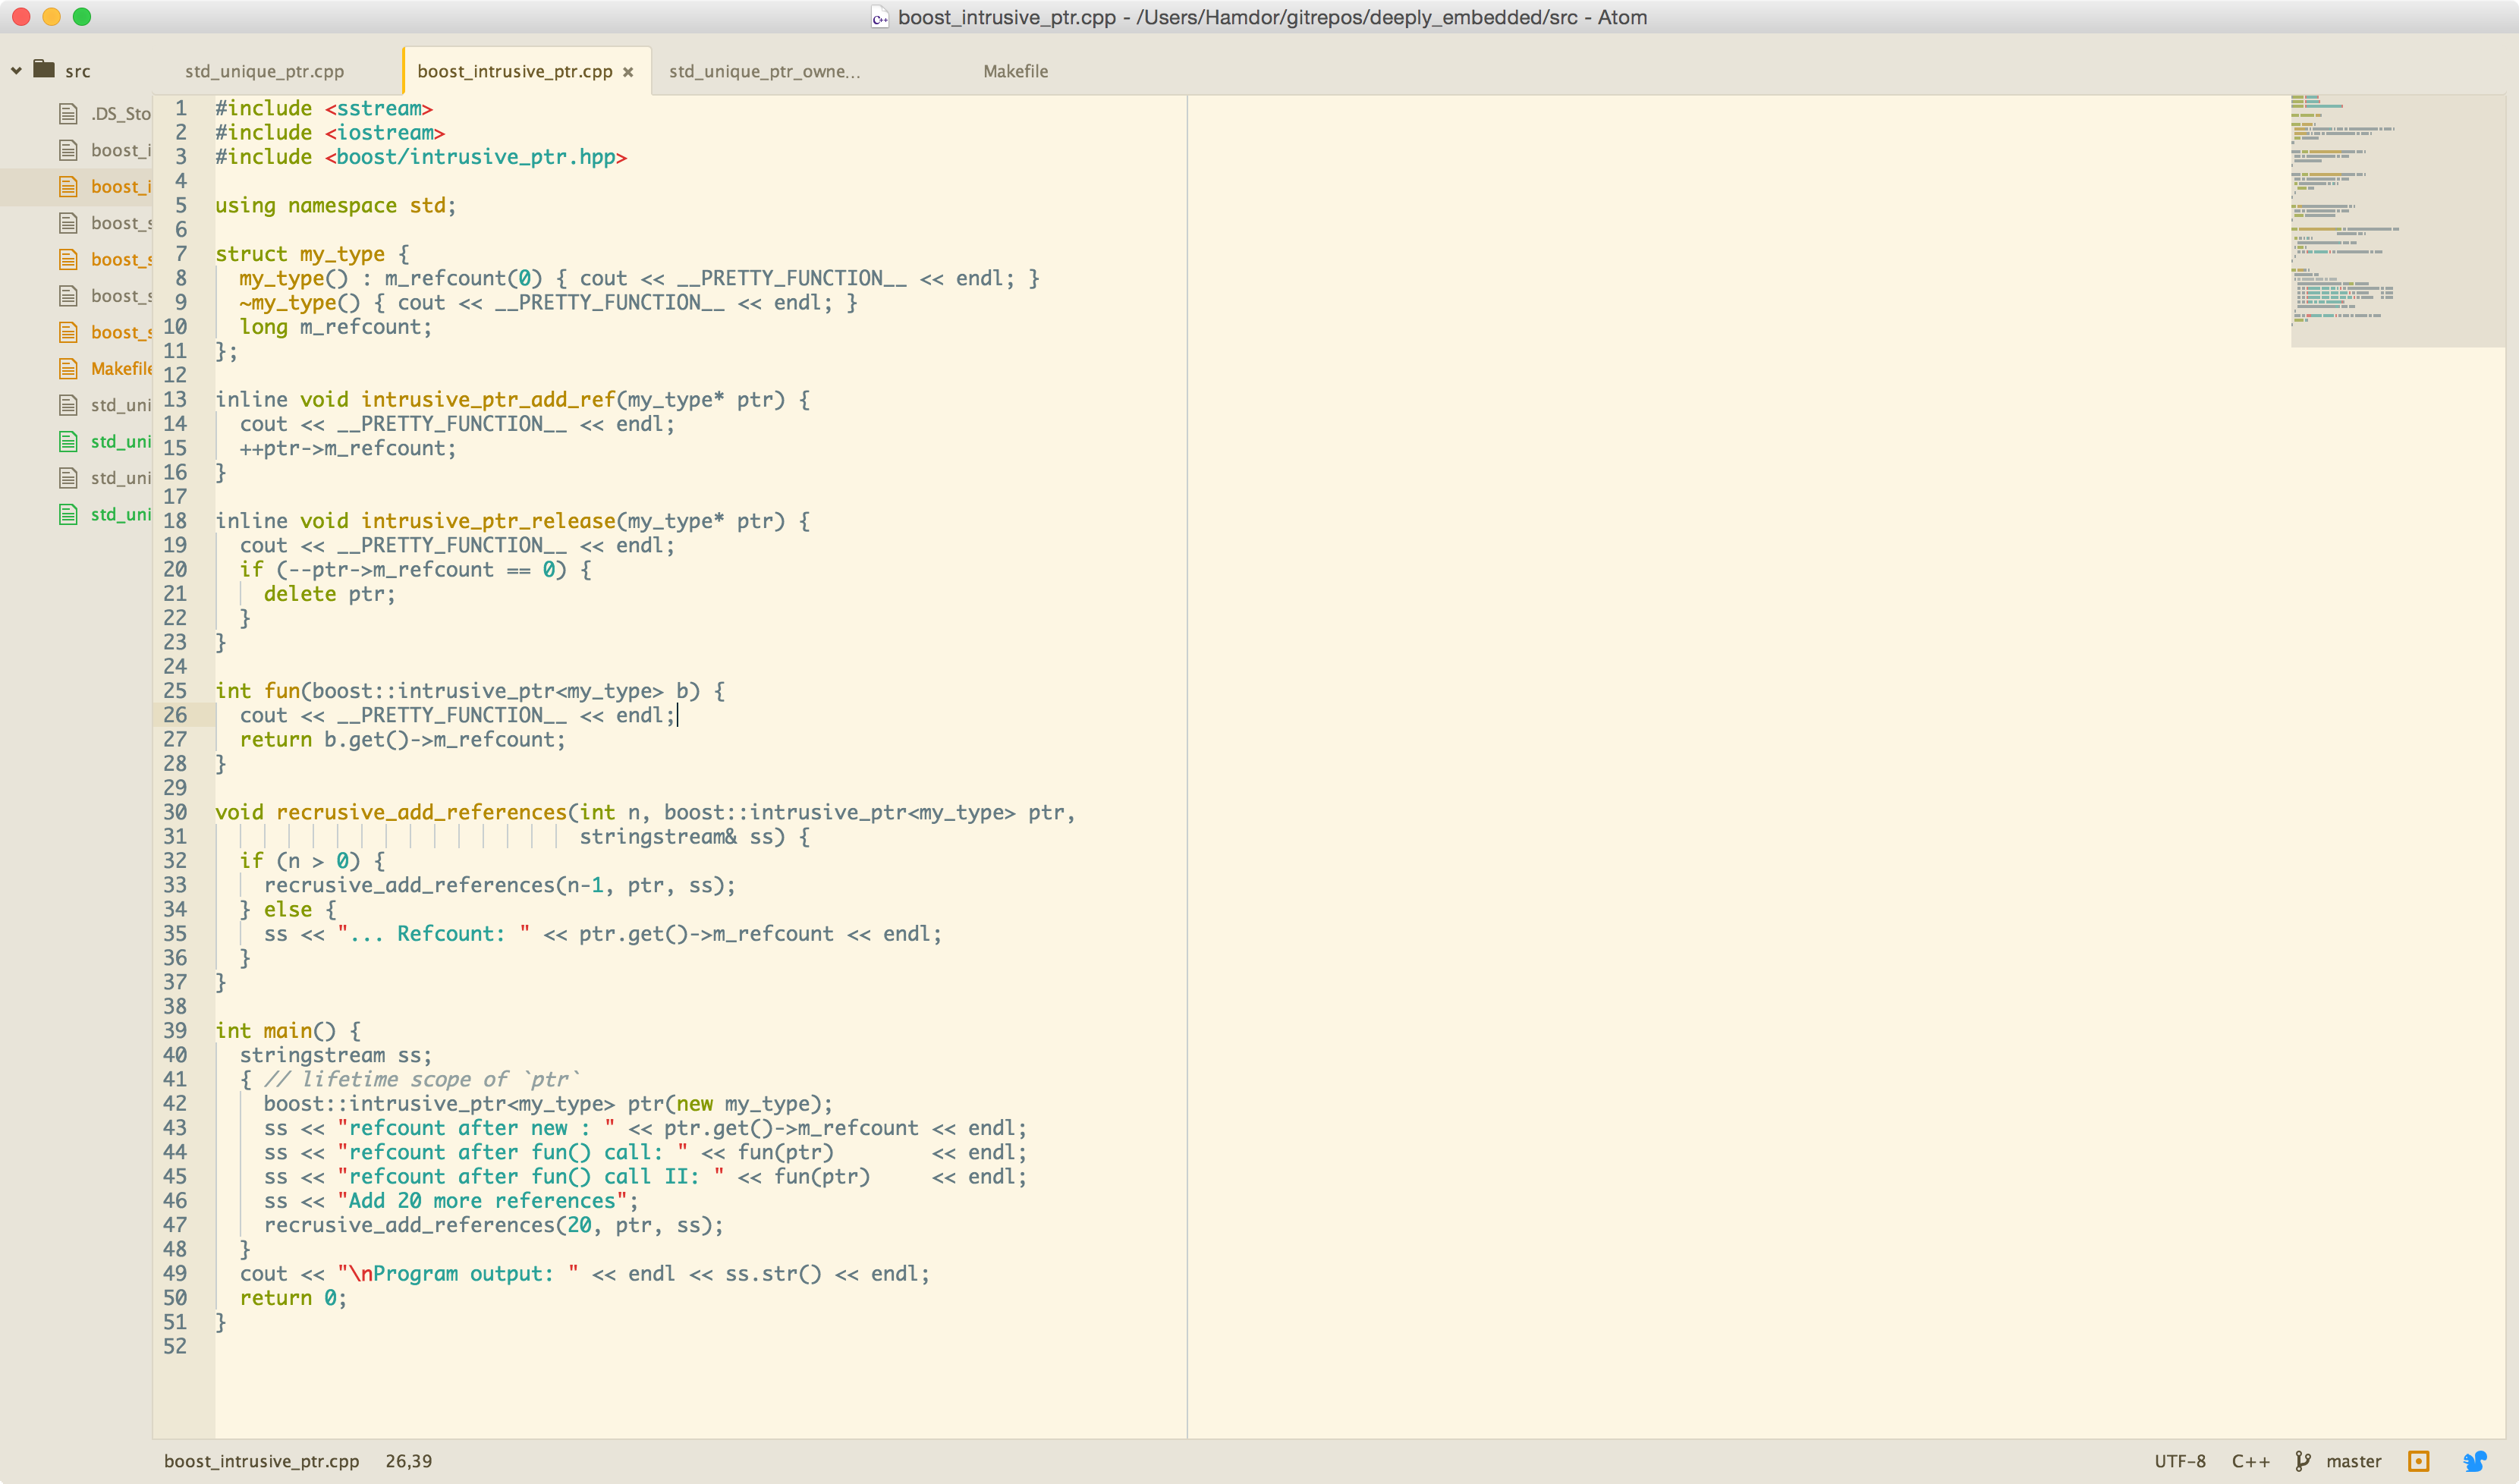
\includegraphics[scale=.21]{intrusive_ptr}	
\end{frame}

% boost::intrusive_ptr Wann?
\begin{frame}
 \frametitle{boost::intrusive\_ptr}
 Vorteile gegenüber Shared Pointern
 \begin{itemize}
  \item Kann auch verwendet werden wenn eine benutzte Bibliothek keine Shared Pointer unterstützt
  \item Light-weight im Vergleich zu Shared Pointer
  \item Geeignet für Performance und Speicher kritische Systeme
 \end{itemize}
 Nachteile gegenüber Shared Pointer
 \begin{itemize}
 	\item Hat immer einen Referenz Counter, kann nicht beliebig abgeschaltet werden
 	\item D.h. nur für Heap Objekte Interessant
 \end{itemize}
\end{frame}

% Implementierung von shared pointern
\begin{frame}
 \frametitle{Implementierung von Shared Pointern}
 \begin{itemize}
 	\item Template Klasse die intern beliebigen Typen speichern kann
 	\item Besteht aus 2 Objekten im Heap
 	\item 1) Referenzzähler
 	\item 2) Pointer auf die Daten
 	\item Shared Pointer auf gleichen PTR teilen sich gleichen Referenzzähler
 \end{itemize}
\end{frame}

% Implementierung von shared pointern
\begin{frame}
 \frametitle{Implementierung von Shared Pointern}
 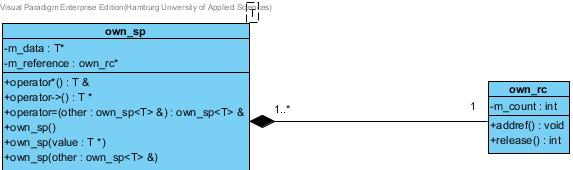
\includegraphics[scale=.6]{own_sp_classdiagram}
\end{frame}

% Implementierung von shared pointern
\begin{frame}
 \frametitle{Implementierung von Shared Pointern}
 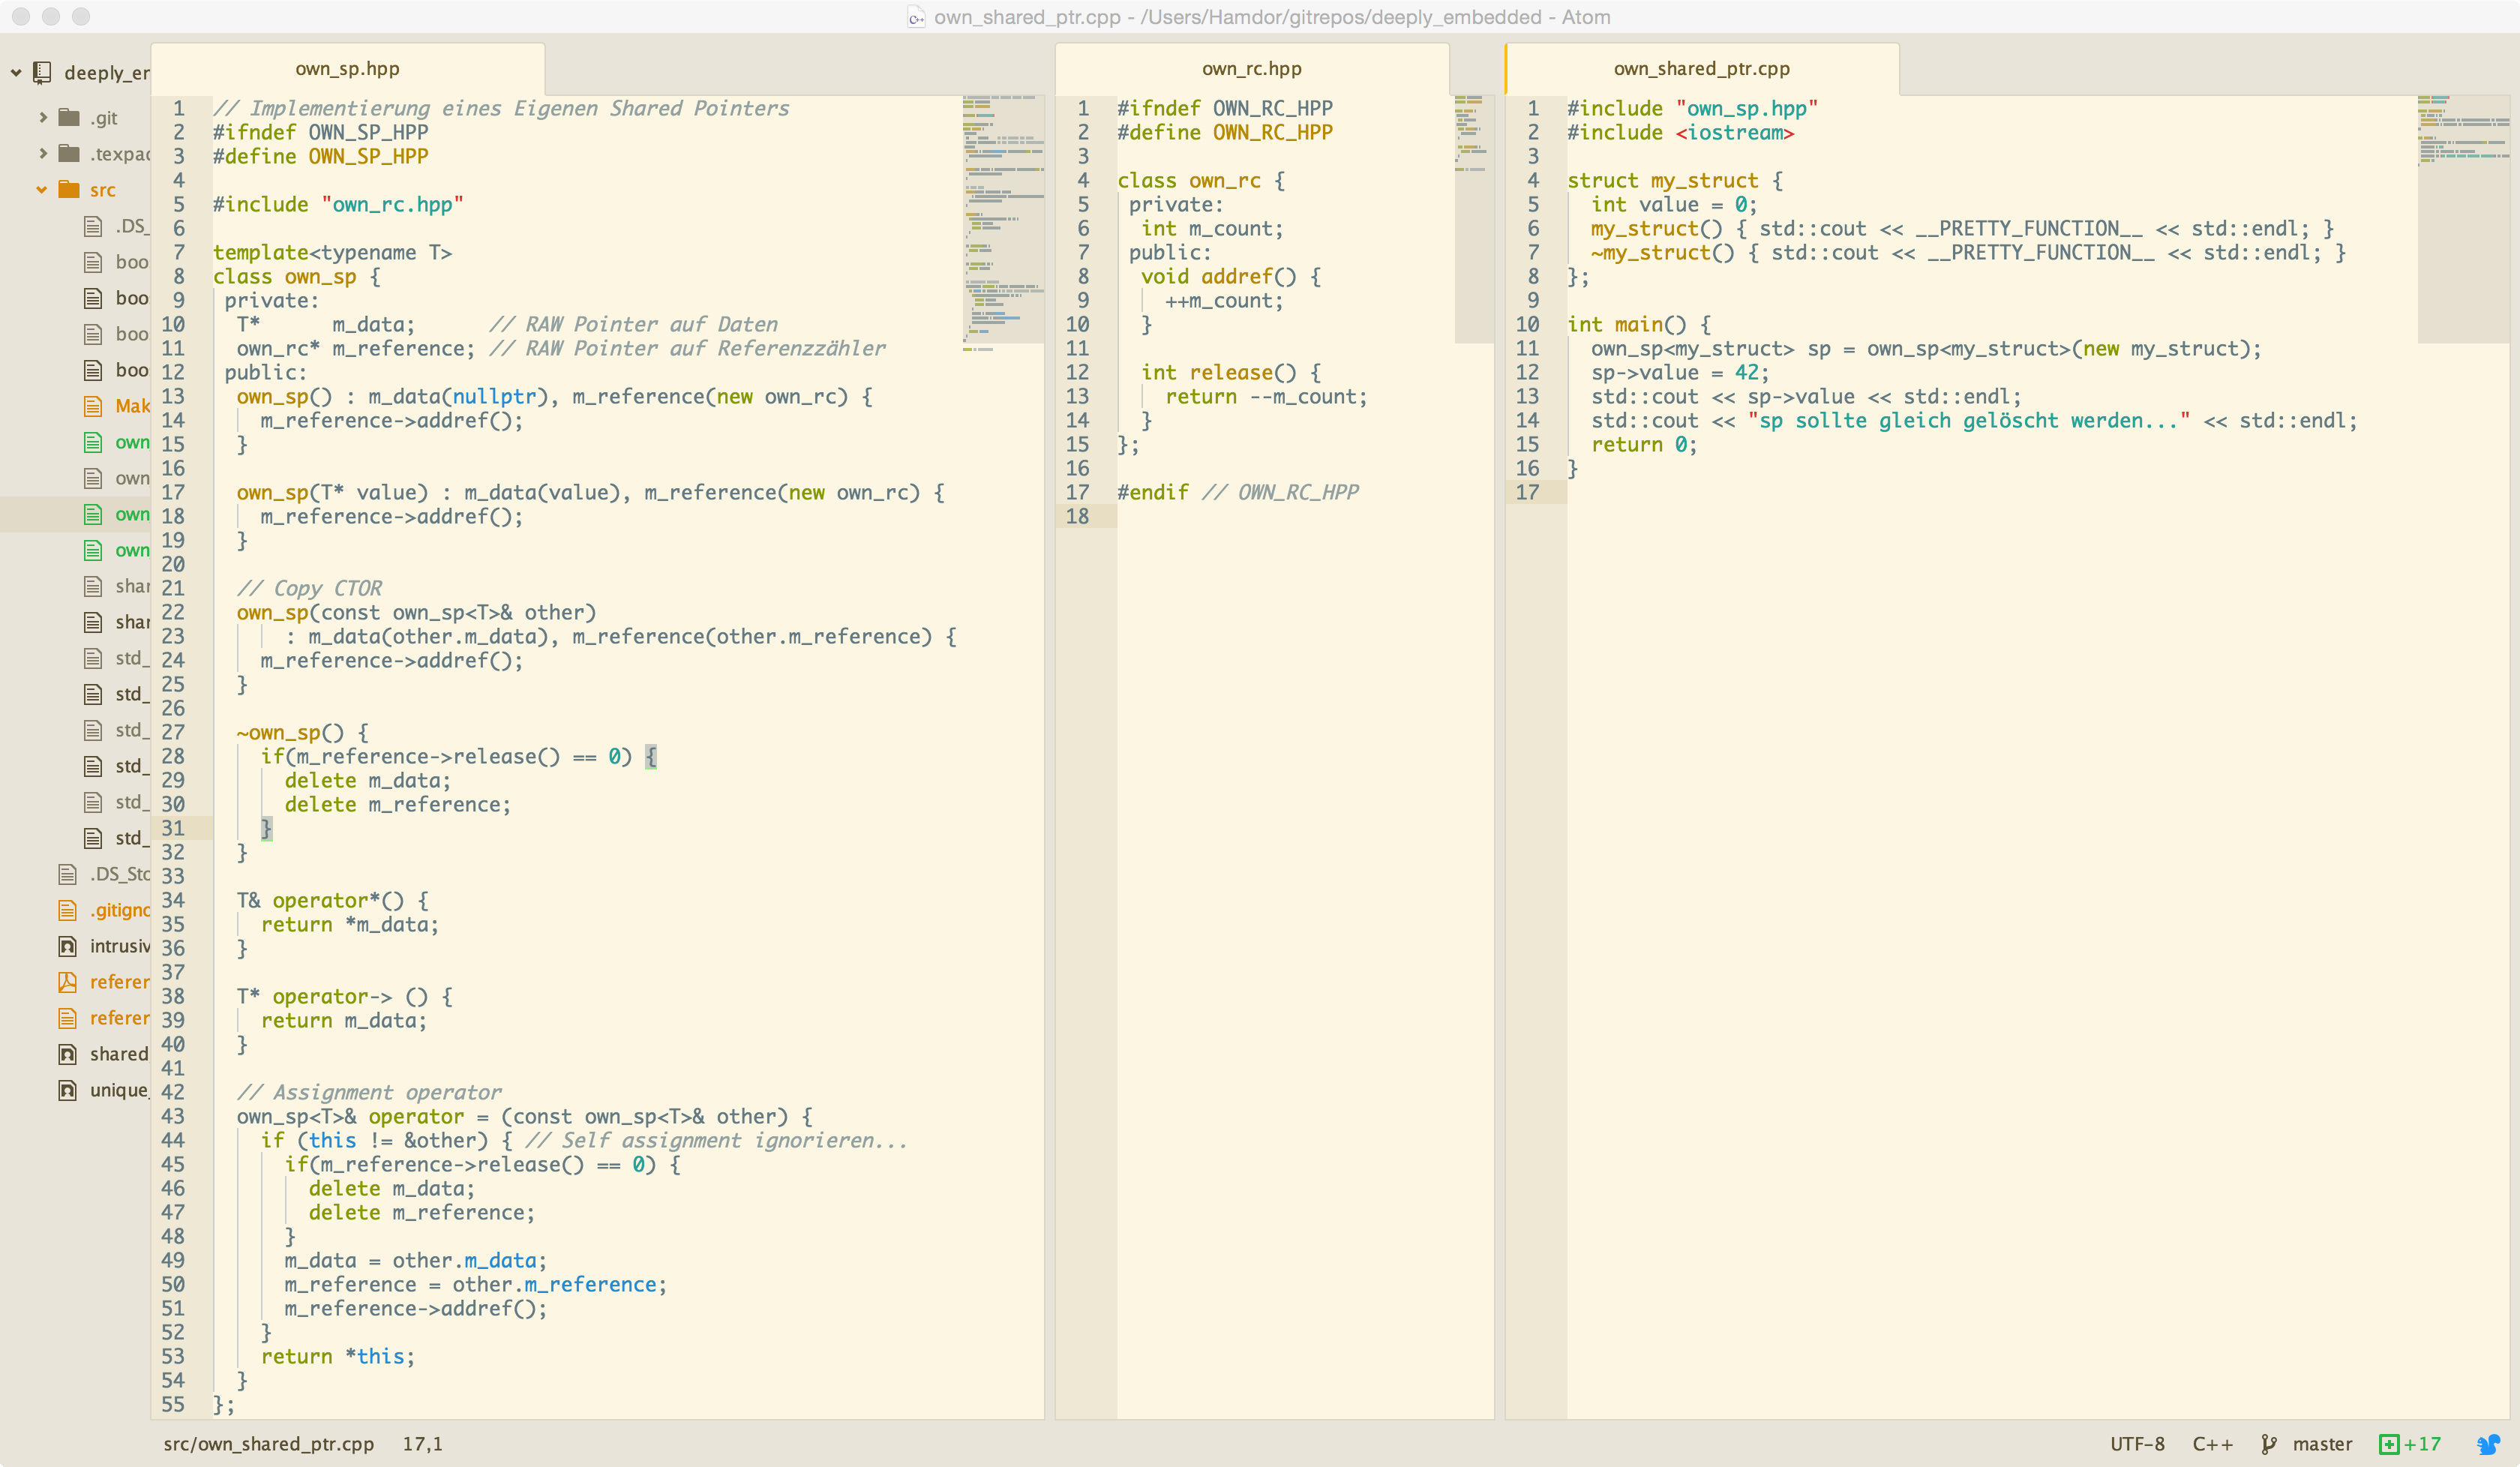
\includegraphics[scale=.2]{own_sp.png}
\end{frame}

\begin{frame}
\center
Source Codes:\\
\textit{https://github.com/Hamdor/WPDE}\\
Gute Hilfen rund um C++:\\
\textit{http://en.cppreference.com/}
\end{frame}

\end{document}
